\documentclass[11pt]{article}

\usepackage{float}
\usepackage{hyperref}
\usepackage{graphicx}
% formatting
\usepackage{fullpage}
\usepackage{verbatim}
\usepackage{moreverb}
\usepackage{minted}
\let\verbatiminput=\verbatimtabinput
\def\verbatimtabsize{4\relax}

\begin{document}
\title{EECS 151/251A FPGA Lab\\
Lab 2: Simulation, Basic FSMs, and Memories}

\author{Prof. Borivoje Nikolic \\
TA: Vighnesh Iyer \\Department of Electrical Engineering and Computer Sciences\\
College of Engineering, University of California, Berkeley}
\date{}
\maketitle

\section{Before You Start This Lab}

Before you proceed with the contents of this lab, we strongly suggest that you look through three documents that will help you better understand some Verilog constructs.

\begin{enumerate}
	\item \textbf{labs\_fa16/docs/Verilog/wire\_vs\_reg.pdf} - The differences between wire and reg nets and when to use each of them.
	
	\item \textbf{labs\_fa16/docs/Verilog/always\_at\_blocks.pdf} - Understanding the differences between the two types of always @ blocks and what they synthesize to.
	
	\item \textbf{labs\_fa16/docs/Verilog/verilog\_fsm.pdf} - An overview of how to create finite state machines in Verilog, specifying their state transitions and machine outputs.

\end{enumerate}

You should go through the \verb|verilog_fsm.pdf| document before doing the FSM part of this lab. The first couple sections of this lab focus on simulation and it would be valuable to read the first two documents before starting.

\subsection{Helpful Hint: Synthesis Warnings and Errors}
At various times in this lab, things will just not work on the FPGA or simulation. To help with debugging, you can run \verb|make synth| in the \verb|lab2/| folder. This will just run \verb|xst| which will only take a few seconds. Then you should run \verb|make report|. In the window that opened, click on \verb|Synthesis Messages| on the left under \verb|Errors and Warnings|. Any synthesis warnings you see here are a possible alert to some issue in your circuit. If you don't understand a warning, ask a TA; it almost always reveals some issue in your RTL.


\section{Lab Overview}

In this lab, we will begin by taking your \verb|tone_generator| design from Lab 1 and simulating it in software. We will learn about using ModelSim to view waveforms and debug your circuits. You will then extend your \verb|tone_generator| to play a configurable frequency square wave and simulate it to check that you have implemented the functionality correctly. You will then construct a state machine that can pull tones to play from a memory block and send them to your \verb|tone_generator| for a specified amount of time each. Finally, you will modify your state machine so that it can be paused, and so it can play the tones and different tempos.

\section{Simulating the tone\_generator from Lab 1}

\subsection{Copying Your Lab 1 Code}

Run \verb|git pull| in your git cloned \verb|labs_fa16| directory to fetch the latest skeleton files.

Begin by copying your \verb|tone_generator| implementation into the \verb|lab2/tone_generator.v| file. Let's run some simulations on the \verb|tone_generator| in software. To do this, we will need to use a Verilog testbench. A Verilog testbench is designed to test a Verilog module by supplying it with the inputs it needs and testing whether the outputs of the module match what we expect.


\subsection{Overview of Testbench Skeleton}
Check the provided testbench skeleton in \verb|lab2/tone_generator_testbench.v| to see the test written for the \verb|tone_generator|. Let's go through what every line of this testbench does.

\begin{minted}{verilog}
`timescale 1ns/1ns
`timescale (simulation step time)/(simulation resolution)
\end{minted}

The timescale declaration needs to be at the top of every testbench file. It provides information to the circuit simulator about the timing parameters of the simulation.

The first argument to the timescale declaration is the simulation step time. It defines the chunks of discrete time in which the simulation should proceed. In this case, we have defined the simulation step time to be one nanosecond. This means that we can advance the simulation time by as little as 1ns at a time.

The second argument to the timescale declaration is the simulation resolution. In our example it is also 1ns. The resolution allows the simulator to model transient behavior of your circuit in between simulation time steps. For this lab, we aren't modeling any gate delays, so the resolution can equal the step time.

\begin{minted}{verilog}
`define SECOND 1000000000
`define MS 1000000
// The SAMPLE_PERIOD corresponds to a 44100 kHz sampling rate
`define SAMPLE_PERIOD 22675.7
\end{minted}

These are some macros defined for our testbench. They are constant values you can use when writing your testbench to simplify your code and make it obvious what certain numbers mean. For example, \verb|SECOND| is defined as the number of nanoseconds in one second. The \verb|SAMPLE_PERIOD| is the sampling period used to sample the square wave at a standard 44100 kHz sample rate.

\begin{minted}{verilog}
module tone_generator_testbench();
	// Testbench code goes here
endmodule
\end{minted}

This module is our testbench module. It is not something actually synthesized to be placed on our FPGA, but rather just a top-level testbench module to be run by our circuit simulator. All your testbench code goes in this module. We will instantiate our DUT (device under test) in this module.

\begin{minted}{verilog}
reg clock;
reg output_enable;
wire sq_wave;
\end{minted}

Here are the inputs and outputs of our \verb|tone_generator|. You will notice that the inputs to the \verb|tone_generator| are declared as \verb|reg| type nets and the outputs are declared as \verb|wire| type nets. This is because we will be driving the inputs in our testbench and we will be monitoring the output.

\begin{minted}{verilog}
initial clock = 0;
always #(30.3/2) clock <= ~clock;
\end{minted}

Here is our clock signal generation code. The clock net needs to be generated in our testbench so it can be fed to the DUT. The initial statement sets the value of the clock net to 0 at the very start of the simulation. The next line toggles the clock net such that it produces a 33Mhz clock signal.

\begin{minted}{verilog}
tone_generator piezo_controller (
    .clk(clock),
    .output_enable(output_enable),
    .square_wave_out(sq_wave)
);
\end{minted}

Now we instantiate the DUT and connect its ports to the nets we have access to in our testbench.

\begin{minted}{verilog}
initial begin
    output_enable <= 0;
    #(500 * `MS);
    output_enable <= 1;
    #(1 * `SECOND);
    $finish();
end
\end{minted}

Here is the body of our testbench. The \verb|initial begin ... end| block specifies the 'main()' function for our testbench. It is the execution entry point for our simulator. In the \verb|initial| block, we can assign the inputs that flow into our DUT using non-blocking (<=) assignments. \\

We can also order the simulator to advance simulation time using delay statements. A delay statement takes the form \verb|#(delay in time steps);|.\\

In this case, we assign \verb|output_enable| to 0 at the start of the simulation, then we let the simulation run for 500ms, then we set \verb|output_enable| to 1, then we let the simulation run for one second. The final statement is called a \verb|system function|. The \verb|$finish()| function tells the simulator to halt the simulation.

\begin{minted}{verilog}
integer file;
initial begin
	file = $fopen("output.txt", "w");
	forever begin
		$fwrite(file, "%h\n", sq_wave);
		#(`SAMPLE_PERIOD);
	end
end
\end{minted}

This piece of code is written in a separate \verb|initial begin ... end| block. The simulator treats both blocks as separate threads that both start execution at the beginning of the simulation and that operate in parallel.\\

This block of code uses two system functions \verb|$fopen() and $fwrite()|, that allow us to write to a file. The \verb|forever begin| construct tells the simulator to run the chunk of code inside it continuously until the simulation ends.\\

The the \verb|forever begin| block, we sample the \verb|sq_wave| output of the \verb|tone_generator| and save it in a file. We sample this value every \verb|`SAMPLE_PERIOD| nanoseconds which corresponds to a 44100 kHz sampling rate. Your \verb|tone_generator|'s output is stored as 1s and 0s in a file that can be translated to sound to hear how your circuit will sound when deployed on the ML505 development board and FPGA.

\subsection{Using TCL scripts (.do files)}

ModelSim, which is our circuit simulator, takes commands from TCL scripts. Take a look at the \verb|lab2/sim/tests/tone_generator_testbench.do| file. Here is a quick description of what is instructs our simulator to do.

\begin{minted}{tcl}
start tone_generator_testbench
add wave tone_generator_testbench/*
add wave tone_generator_testbench/piezo_controller/*
run 10000ms
\end{minted}

We begin by issuing the \verb|start| command to the simulator. This instructs the simulator to scan a list of Verilog source files provided to it to find a module named \verb|tone_generator_testbench|. This module name must match exactly the module name of your top-level testbench module. The simulator loads and elaborates this module so that its ready to simulate/execute.\\

The two \verb|add_wave| commands are important. By default, the simulator when running the simulation of our circuit will not log the values of the signals in our testbench or DUT unless we tell it to. These lines tell the simulator to store and log the values of the signals directly inside the \verb|tone_generator_testbench| module. The \verb|*| tells the simulator to log all signals directly in the \verb|tone_generator_module|. The second line allows us to log the signals in a submodule of the main testbench module. Observe that \verb|piezo_controller| is the instance name of the \verb|tone_generator| instance in the testbench module.\\

Finally, the \verb|run (time)| command tells the simulator to jump to the \verb|initial begin| blocks in the testbench and actually run the simulation. The time specification (in our case 10000ms = 10s) gives the simulator an upper bound on the simulation time. The simulator won't simulate more than 10 seconds of circuit behavior. If the simulator hits the \verb|$finish()| function before the 10 second timeout is up, it will stop simulation at that moment.

\subsection{Running ModelSim}

With all the details out of the way, let's actually run a simulation. Go to the \verb|lab2/sim| directory and run \verb|make|. After some time the simulation will finish.

\subsection{Viewing Waveforms}

Let's take a look at the data that the simulator collected. Run the viewwave script as such:\\

\verb|./viewwave results/tone_generator_testbench.wlf &|

The results of the simulation and the logged signals are stored in a \verb|.wlf| file. This command should open that file in the ModelSim Wave Viewer.

You should see a window like this:

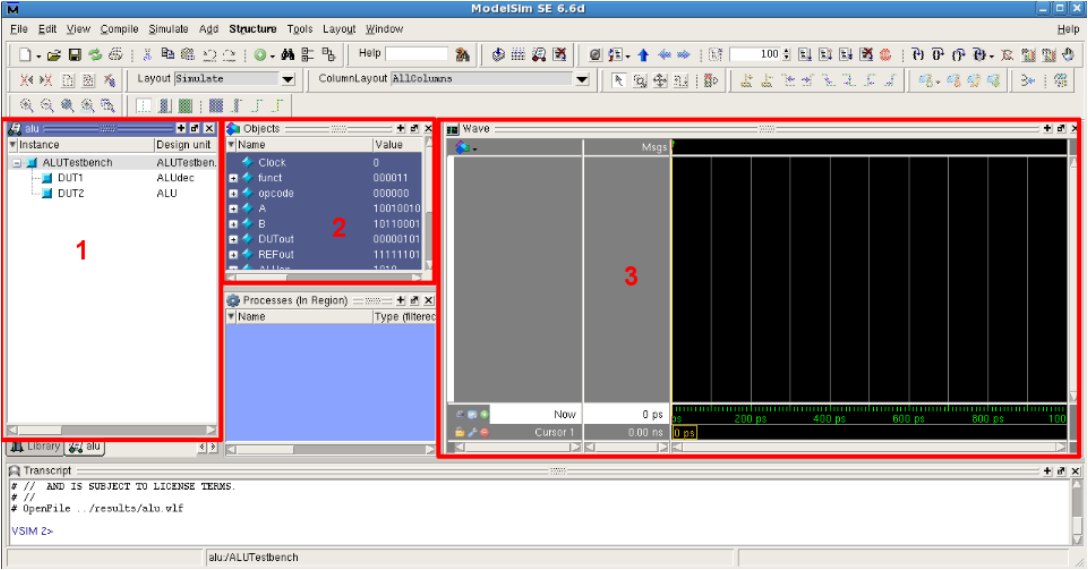
\includegraphics[width=\textwidth]{images/modelsim.png}

Let's go over the basics of ModelSim. The boxed screens are:

\begin{enumerate}
	\item List of the module involved in the testbench. You can select one of these to have its signals show up in the object window.
	\item \textbf{Object Window} - this lists all the wires and regs in your module. You can add signals to the waveform view by selecting them, right-clicking, and doing \verb|Add Wave|.
	\item \textbf{Waveform Viewer} - The signals that you add from the object window show up here. You can navigate the waves by searching for specific values or going forward or backward one transition at a time. The x-axis represents time.
\end{enumerate}

Add the \verb|clock, output_enable,| and \verb|sq_wave| signals to the waveform viewer. Click anywhere on the waveform viewer to set your cursor and use the \verb|O| and \verb|I| keys to zoom in and out. Zoom out all the way.

You should be able to see the clock oscillate at the frequency specified in the testbench. You should also see the \verb|output_enable| signal start at 0 and then become 1 after 500 ms. However, you will see that the \verb|sq_wave| signal is just a red line. What's going on?

\subsection{Fixing the Undefined clock\_counter}

Take a look at the \verb|clock_counter| in your \verb|tone_generator| module. Plot the signal in your waveform viewer. You will notice it's also a red line. Red lines in ModelSim indicate undefined signals (indicated in Verilog as the letter \verb|x|). \\

Blue lines in ModelSim indicate high-impedance (unconnected) signals. High-impedance is defined in Verilog as the letter \verb|z|. We won't be using high-impedance signals in our designs, but blue lines in ModelSim indicate something in our testbench isn't wired up properly.\\

Going back to the red line for \verb|clock_counter|: this is caused because at the start of simulation, the value sitting inside the \verb|clock_counter| register is unknown. It could be anything! Since we don't have an explicit reset signal for our circuit to bring the \verb|clock_counter| to a defined value, it is unknown for the entire simulation.\\

Let's fix this. In the future we will use a reset signal, but for now let's use a simpler technique. In \verb|lab2/tone_generator.v| modify the \verb|reg [x:0] clock_counter| line to read \verb|reg [x:0] clock_counter = 0| instead. This implicitly tells the simulator that the initial simulation value for this register should be 0. For this lab, when you add new registers in your \verb|tone_generator| or any other design module, you should instantiate them to their default value in the same way.\\

Now run the simulation again.

\subsubsection{Helpful Tip: Reloading ModelSim .wlf}

When you re-run your simulation and you want to plot the newly generated signals in ModelSim, you don't need to close and reopen ModelSim. Instead click on the 'Reload' button on the top toolbar which is to the right of the 'Save' button.

\subsection{Listen to Your Square Wave Output}

Take a look at the file written by the testbench located at \verb|lab2/sim/build/output.txt|. It should be a sequence of 1s and 0s that represent the output of your \verb|tone_generator|. I've written a Python script that can take this file and generate a \verb|.wav| file that you can listen to.\\

Go to the \verb|lab2/| directory and run the command:\\

\verb|python audio_from_sim.py sim/build/output.txt|\\

This will generate a file called \verb|output.wav|. Run this command to play it:\\

\verb|play output.wav|

You should hear a 440Hz square wave for 1 second after half a second of silence.

\subsection{Playing with the Testbench}

Play around with the testbench by altering the clock frequency, changing when you turn on \verb|output_enable| and verify that you get the audio you expect. For checkoff be able to answer the following question and demonstrate understanding of basic simulation

\begin{enumerate}
	\item If you increase the clock frequency, would you expect the tone generated by your \verb|tone_generator| to be of higher pitch or lower pitch from 440Hz? Why? Show audio evidence of this from the simulation.
\end{enumerate}

\section{Design a Configurable Frequency tone\_generator}

Let's extend our \verb|tone_generator| so that it can play different notes. Add a 24-bit input to the \verb|tone_generator| module called \verb|tone_switch_period|. Note you will also have to modify your \verb|clock_counter| to be 24 bits wide.\\

The \verb|tone_switch_period| describes how many clock cycles you should hold the value of your square wave before inverting it. For example a \verb|tone_switch_period| of 37500 tells us to invert the square wave every 37500 clock cycles, which for a 33 Mhz clock translates to a 440 Hz square wave.

You may have to modify the architecture of your \verb|tone_generator| to accommodate this new input signal. You should reset the internal clock counter every \verb|tone_switch_period| cycles and should invert the square wave output. Remember to initialize any new registers declared in your \verb|tone_generator| to their default value to prevent unknowns during simulation.

\section{Simulating and Debugging Your New tone\_generator}

Now, extend the testbench to work with this new input signal. Add a new 24-bit reg to the testbench. Set \verb|output_enable| to 1 at the start of the simulation. Then set the \verb|tone_switch_period| of the DUT and run the simulation for some time (using a delay statement). Then change the \verb|tone_switch_period| again and run the simulation for some more time.\\

Inspect the waveform and debug your \verb|tone_generator| if you detect any bugs. Then use the same Python script to generate an audio file to listen to your \verb|tone_generator|.

I suggest using \url{http://onlinetonegenerator.com/} to generate sample square wave tones and making sure your tones match.\\

Create a testbench that plays some simple melody that you define and show the TA before proceeding further.

\section{Try tone\_generator on the FPGA}
Modify the top-level Verilog module \verb|ml505top.v| to include the new input to the \verb|tone_generator|. You can tie the new input to any value you want.

Run the usual \verb|make| process and then \verb|make impact| to put your new \verb|tone_generator| on the FPGA. It should work as it did before.

\section{Introduction to Inferred Asynchronous Memories}



\section{Design of the music\_streamer FSM}

\section{Simulating the music\_streamer}

\section{Adding Tempo Variations to the music\_streamer}

\section{Try it on the FPGA!}
\end{document}